% !TEX TS-program = pdfLaTeX+shellescape
% !TEX encoding = UTF-8 Unicode

\documentclass{standalone}
\usepackage{pgfplots}
\pgfplotsset{compat=1.17}

\begin{document}
    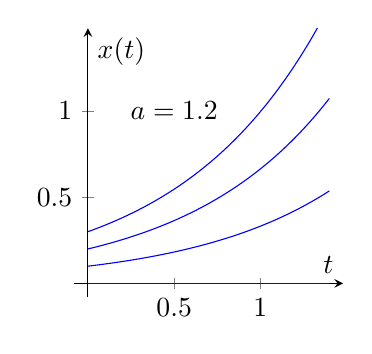
\begin{tikzpicture}[baseline]
        \begin{axis}[
            scale=0.6, % scale
            % view = {0}{90},
            xmin=-0.08,xmax=1.48,ymin=-0.08,ymax=1.48, % range of plot
            % legend style={at={(axis cs: 1,0)}, anchor=south east}, % position of legends
            % unit vector ratio = {1, 1, 1}, % aspect ratio
            unit vector ratio = {1, 1}, % aspect ratio
            axis lines = middle, % middle or box
            %axis x line = bottom, % top, middle, bottom, none: axis x line* = ... removes arrow heads
            %axis y line = left, % left, center, right, none: axis y line* = ... removes arrow heads
            xlabel = {$t$}, ylabel = {$x(t)$}, % axis labels 
        ]
            % \addplot3[blue, quiver={u={y}, v={-x}}, domain=-1.5:1.5, y domain=-1.5:1.5, samples=12, -latex] (x, y, 0);
            \addplot[blue, domain=0:1.4, samples=100]({x}, {0});
            \addplot[blue, domain=0:1.4, samples=100]({x}, {0.1*exp(1.2*x)});
            \addplot[blue, domain=0:1.4, samples=100]({x}, {0.2*exp(1.2*x)});
            \addplot[blue, domain=0:1.4, samples=100]({x}, {0.3*exp(1.2*x)});
            \node at (0.5, 1.0) {$a=1.2$};
        \end{axis}
    \end{tikzpicture}
    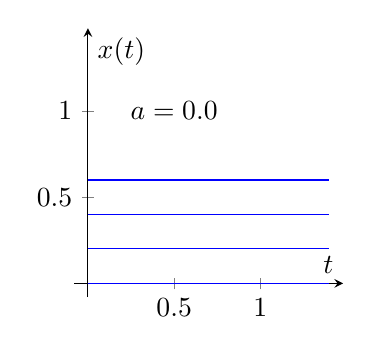
\begin{tikzpicture}[baseline]
        \begin{axis}[
            scale=0.6, % scale
            % view = {0}{90},
            xmin=-0.08,xmax=1.48,ymin=-0.08,ymax=1.48, % range of plot
            % legend style={at={(axis cs: 1,0)}, anchor=south east}, % position of legends
            % unit vector ratio = {1, 1, 1}, % aspect ratio
            unit vector ratio = {1, 1}, % aspect ratio
            axis lines = middle, % middle or box
            %axis x line = bottom, % top, middle, bottom, none: axis x line* = ... removes arrow heads
            %axis y line = left, % left, center, right, none: axis y line* = ... removes arrow heads
            xlabel = {$t$}, ylabel = {$x(t)$}, % axis labels 
        ]
            % \addplot3[blue, quiver={u={y}, v={-x}}, domain=-1.5:1.5, y domain=-1.5:1.5, samples=12, -latex] (x, y, 0);
            \addplot[blue, domain=0:1.4, samples=100]({x}, {0});
            \addplot[blue, domain=0:1.4, samples=100]({x}, {0.2});
            \addplot[blue, domain=0:1.4, samples=100]({x}, {0.4});
            \addplot[blue, domain=0:1.4, samples=100]({x}, {0.6});
            \node at (0.5, 1.0) {$a=0.0$};
        \end{axis}
    \end{tikzpicture}
    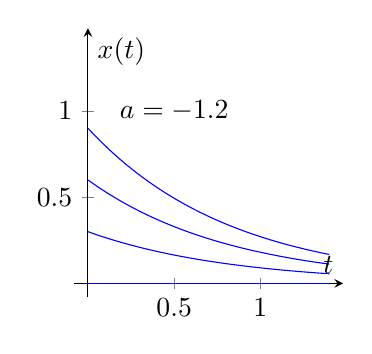
\begin{tikzpicture}[baseline]
        \begin{axis}[
            scale=0.6, % scale
            % view = {0}{90},
            xmin=-0.08,xmax=1.48,ymin=-0.08,ymax=1.48, % range of plot
            % legend style={at={(axis cs: 1,0)}, anchor=south east}, % position of legends
            % unit vector ratio = {1, 1, 1}, % aspect ratio
            unit vector ratio = {1, 1}, % aspect ratio
            axis lines = middle, % middle or box
            %axis x line = bottom, % top, middle, bottom, none: axis x line* = ... removes arrow heads
            %axis y line = left, % left, center, right, none: axis y line* = ... removes arrow heads
            xlabel = {$t$}, ylabel = {$x(t)$}, % axis labels 
        ]
            % \addplot3[blue, quiver={u={y}, v={-x}}, domain=-1.5:1.5, y domain=-1.5:1.5, samples=12, -latex] (x, y, 0);
            \addplot[blue, domain=0:1.4, samples=100]({x}, {0});
            \addplot[blue, domain=0:1.4, samples=100]({x}, {0.3*exp(-1.2*x)});
            \addplot[blue, domain=0:1.4, samples=100]({x}, {0.6*exp(-1.2*x)});
            \addplot[blue, domain=0:1.4, samples=100]({x}, {0.9*exp(-1.2*x)});
            \node at (0.5, 1.0) {$a=-1.2$};
        \end{axis}
    \end{tikzpicture}
\end{document}